\chapter{Group-V monolayers as versatile platforms for topological phases}
\label{ch:tci}
One of the most natural extensions of the ten-fold way is to include spatial symmetries represented by unitary operators, which are inherently present in crystalline solids. Those symmetries are point group symmetries, such as rotations and reflections, which leave at least one point in space invariant or space-group symmetries being the combinations of translational symmetry and symmetry operations like screw axes or glide planes. For 3D systems, a combination of 32 crystallographic point groups and 14 Bravais lattices leads to 230 space groups. Imposing crystal symmetries may have two possible outcomes on the ten-fold way: 
\begin{enumerate}[label=\textbf{\arabic*.}]
\item topological classification remains the same, but topological invariants are easier to calculate~\cite{PhysRevB.86.115112},
\item spatial symmetries give rise to novel topological phases, hence the classification has to be refined.
\end{enumerate}
For instance, the Fu-Kane formula relies on the presence of inversion symmetry and simplifies the computation of the $\mathbb{Z}_2$ invariant by taking into account only the parity eigenvalues at TRIMs~\cite{FuKane2007}. On the other hand, the concept of topological crystalline insulators (TCIs) stems solely from the presence of spatial symmetries~\cite{FuTCI2011}. TCIs, which are a subset of symmetry-protected topological phases, cannot be adiabatically deformed to an atomic insulator without breaking the relevant symmetries. Given the complexity of the problem, the full classification of TCIs remains an open question. So far, the classification of TCIs in all 230 non-magnetic and 1651 magnetic space groups has been achieved for systems where symmetry indicators can be employed~\cite{Po2017, Bradlyn17, watanabe2018structure, Tang2019} (this approach is discussed in more details in Chapter~\ref{ch:oals}). For more general symmetry configurations, a partial classification was provided in Ref.~\cite{Slager2013}, but most of the works concerns the systems with point group symmetries~\cite{RevModPhys.88.035005, PhysRevB.90.165114, PhysRevB.95.235425, PhysRevB.93.045429}.

There are also further distinctions in the formulation of the bulk-boundary correspondence for TIs and TCIs. For TIs equipped with internal symmetries, gapless boundary modes are present at every boundary. In contrast, TCIs exhibit surface/edge states only at the boundaries which are unchanged upon the action of crystal symmetries. Therefore, the absence of protected modes in TCIs does not necessary indicates trivial bulk topology. It is the case for inversion-symmetric systems for which no boundaries respecting the inversion can exist\footnote{Suppose we have a material with inversion symmetry $\mathcal{I}$ in the bulk; if there is an atom at a point $(x, y, z)$, then inversion implies the presence of another, identical one at $(-x, -y, -z)$, which is not true for \emph{any} surface.}. In addition, a robustness against disorder can be seen from a slightly different perspective. Spatial disorder always breaks the crystal symmetries, but gapless boundary states may avoid the Anderson localization if the symmetries are retained on average~\cite{Diez_2015, PhysRevB.88.125129}. Such situation is similar to weak TIs~\cite{PhysRevLett.98.106803}, where the gapless surface states are protected by a discrete translation symmetry of a shift by one layer along the stacking direction. In both cases, protected conducting states are present if the disorder breaks the symmetries locally, but preserves them at the macroscopical level. A notion of delocalization via average symmetry was formulated within the non-linear $\sigma$ model~\cite{fu2012topology} and, subsequently, confirmed numerically~\cite{PhysRevLett.108.076804, PhysRevLett.110.236803, PhysRevB.89.155315}.

The first family of TCI materials in IV-VI semiconductors with rock-salt structure was predicted in 2012~\cite{HsiehTCI2012}. In the paradigmatic tin telluride (SnTe), the mirror symmetry with respect to the (110) mirror planes protects the conducting surface states, which was verified by angle-resolved photoemission spectroscopy (ARPES)~\cite{Tanaka2012}. A TCI phase was also found in Pb$_{1-x}$Sn$_x$Se~\cite{Dziawa2012}, Pb$_{1-x}$Sn$_x$Te~\cite{Xu2012, PhysRevB.87.155105} and Pb$_{1-x}$Sn$_{x}$Se~\cite{PhysRevB.87.115106} alloys. Another class of TCI protected by glide reflection and time-reversal symmetry was discovered in KHgSb~\cite{Mae1602415}, just after the theoretical proposition of hourglass fermions~\cite{Wang2016} relying on non-symmorphic symmetries. For 2D systems, however, experimental evidences for TCI phases enforced by the mirror symmetry along $z$ direction, $\mathcal{M}_z$, are still lacking; this is mostly due to the fact that $\mathcal{M}_z$ is broken for layers grown on a substrate~\cite{Shen2014}. So far, a list of material candidates includes multilayer thin films of XY semiconductors (X = Ge, Sn, Pb and Y = S, Se, Te) below a critical thickness~\cite{Liu2014, PhysRevB.90.045309, C7CP04679K}, electron-doped TlM ($M$ = S and Se) (110) monolayer~\cite{Niu2015}, PbPo monolayer~\cite{C6TC03197H}, graphene multilayers~\cite{PhysRevLett.114.226802} or even quantum wells consisting of trivial insulators (Sn/Pb)Te and Na(Cl/Br)~\cite{Niu_2016}. 

In the following, we examine the properties of atomically thin layers of bismuth (Bi) and antimony (Sb), which are predicted to be excellent tunable platforms hosting distinct topological phases ~\cite{Hsu2016, Wang_2017}. To do so, we investigate these monolayers within the effective tight-binding model~\cite{Liu:Allen} and characterize TI and TCI phases, together with topological phase transitions induced by doping, external perturbations such as fields or strain and coupling to a substrate. In addition to computing relevant topological invariants, we employ methods based on quantum entanglement, namely entanglement entropy and entanglement spectrum, which in case of gapped, free-fermionic systems, can be deduced from a single-particle correlation matrix~\cite{Peschel}. We illustrate that entanglement measures are useful not only in studying toy models, but can be also a viable complementary tool for realistic Hamiltonians. As an introduction, in Section~\ref{sec:mirror} we discuss the role of mirror symmetry in the protection of surface states for a simple cubic lattice and define a suitable topological invariant, which can be also used for two-dimensional systems. Then, in Section~\ref{sec:entanglement}, we shortly review how entanglement measures may be applicable in the realm of topological non-interacting systems. Section~\ref{sec:bismuth-antimony} is dedicated to the properties of buckled free-standing monolayers of Bi and Sb, while Section~\ref{sec:bismuthene-antimonene} addresses their completely flat counterparts. At the end, in Section~\ref{sec:sic} we consider the effect of the experimentally relevant silicon carbide (SiC) substrate on the properties of studied systems. 

\section{Mirror symmetries and the mirror Chern number}
\label{sec:mirror}
Similarly to Chern number or $\mathbb{Z}_2$ invariant, we can define new topological invariants for systems in which the gapless boundary modes are protected by a mirror symmetry. Suppose we have a 3D gapped system with time-reversal symmetry and reflection symmetry with respect to a mirror plane, see Fig.~\ref{fig:3d_mirror}. The mirror operator $\mathcal{M}$ can be written as a product of the inversion symmetry $\mathcal{I}$ and $C_2$ describing a rotation by $\pi$ around an axis perpendicular to the mirror plane, $\mathcal{M} = \mathcal{I} C_2$. Crystalline symmetry acts non-locally in real space, but also relates different parts of the BZ to each other. For instance, a reflection around $z$-axis sends the coordinates $(x, y, z) \rightarrow (x, y, -z)$ and transforms $(k_x, k_y, k_z) \rightarrow (k_x, k_y, -k_z)$. In the case of spinful systems, $\mathcal{M}$ also acts on spin degrees of freedom and satisfies $\mathcal{M}^2 = - 1$. We then see that the Bloch Hamiltonian commutes with the mirror operator $\mathcal{M}$ in the mirror-invariant planes, $k_z = 0$ and $k_z = \pi$. 

\begin{figure}[H]
\centering
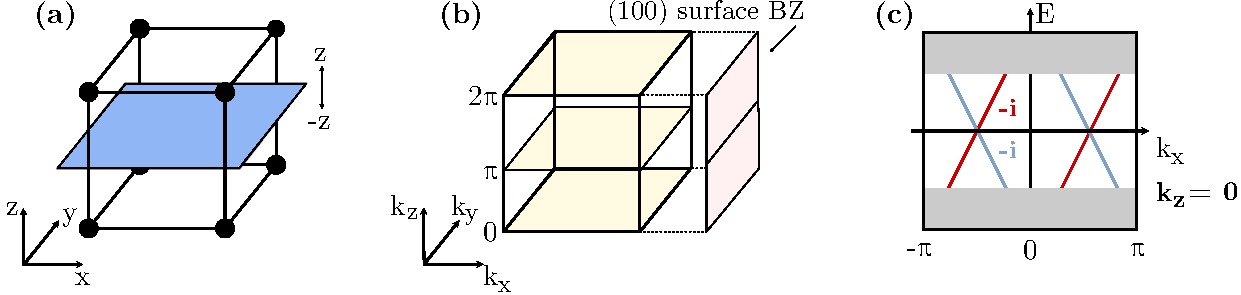
\includegraphics[width= \textwidth]{tci_mirror.pdf}
\caption[Mirror-symmetric 3D cubic lattice]{\textbf{(a)} 3D cubic lattice with a mirror symmetry along $z$-axis, \textbf{(b)} corresponding Brillouin zone with mirror-invariant planes (denoted by a light yellow color) and \textbf{(c)} schematic surface band structure for a time-reversal topological crystalline insulator with $\mathcal{C}_{\mathcal{M}} = 2$ along the projection of the $k_z = 0$ mirror-invariant plane. Two planes at $k_z = 0$ and at $k_z = \pi$ are left invariant upon the action of the mirror symmetry $\mathcal{M}$, hence they may be used to define the mirror Chern number $\mathcal{C}_{\mathcal{M}}$. A $\mathcal{C}_{\mathcal{M}} =2 $ implies the existence of two pairs of chiral modes along mirror-symmetric lines in the surface BZ constructed from the projection of the mirror-invariant planes.}
\label{fig:3d_mirror}
\end{figure}

The Bloch states $\ket{u_{\mathbf{k} n}}$ in these planes can be decomposed into two groups with mirror eigenvalues $\pm \mathrm{i}$~\footnote{For spinless fermions, the mirror eigenvalues are $\pm 1$.}
\begin{equation}
\mathcal{M} \ket{ u^{\pm}_{\mathbf{k} n }} = \pm \, \mathrm{i} \ket{ u^{\pm}_{\mathbf{k} n}}
\end{equation}
where the momentum $\mathbf{k}$ is restricted to the mirror planes. The two mirror eigenspaces are decoupled; moreover, if the time-reversal symmetry is present, both subspaces have the same dimension. Each block separately breaks the time-reversal symmetry, hence we can assign a non-vanishing Chern number with each of them. Additionally, TR enforces the total Chern number to be zero, $\mathcal{C}_{+} +  \mathcal{C}_{-} = 0$; $\mathcal{T}$ implies the Berry curvature to be an odd function of the crystal momentum, $\mathcal{F} (\mathbf{k} ) = - \mathcal{F} (- \mathbf{k} )$, and as a consequence, the integral over the whole BZ vanishes. In analogy to the spin Chern number for QSH states, we can define the mirror Chern number as
\begin{equation}
\mathcal{C}_{\mathcal{M}} = \frac{\mathcal{C}_{+} -\mathcal{C}_{-}}{2}.
\label{eq:mirror_chern}
\end{equation}
Non-zero mirror Chern number implies the existence of gapless Dirac cones only on surfaces preserving reflection symmetry, with the total number of protected Dirac cones depending on the considered surface. To understand the nature of these surface states in more details, let us assume non-trivial $\mathcal{C}_{\mathcal{M}}$ at $k_z = 0$ plane, illustrated in Fig.~\ref{fig:3d_mirror}~(c). $\mathcal{C}_{\mathcal{M}} = 2$ imposes the presence of two pairs of counterpropagating states along $k_z =0$\footnote{In general, the mirror Chern number $|\mathcal{C}_{\mathcal{M}}|$ gives rise to $\mathcal{C}_{\mathcal{M}}$ pairs of chiral states.}. At $k_z = 0$, all states are eigenstates of the mirror symmetry $\mathcal{M}$ and the crossing occurs only between left- and right-movers, which belong to different mirror subspaces. This prevents a gap from opening and the crossing points are symmetry-protected. Away from $k_z = 0$, however, the states do not have a well-defined mirror eigenvalue and are generically gapped. If $\mathcal{C}_{\mathcal{M}}$ is odd (and TR symmetry is present), the system is a conventional topological insulator with an odd number of Dirac cones in the surface BZ, which are located at time-reversal invariant momenta. On the contrary, even $\mathcal{C}_{\mathcal{M}}$ implies an even number of Dirac cones existing only on mirror-symmetric surfaces, but at generic momenta~\cite{HsiehTCI2012}. Similar intuition applies to two-dimensional systems as well. Indeed, the $2$D lattice defined in the $xy$ plane has automatically the $\mathcal{M}}_z$ symmetry and it consists of a single mirror plane located just at $z = 0$. 

\section{Entanglement measures}
\label{sec:entanglement}
Subtle non-local correlations encoded in the topological ground state wavefunctions can be studied by employing the tools at intersection between quantum information theory and condensed matter physics. In particular, the entanglement entropy (EE) and the entanglement spectrum (ES) are amongst the most successful methods that allow to quantify entanglement in many-body systems (for more details on entanglement measures, we refer to the comprehensive review in Ref.~\cite{RevModPhys.80.517}), which we briefly discuss in this Section.

\subsection{Von Neumann entanglement entropy}
Quantum correlations and superposition may prevent an observer from having a simple wavefunction description of a subpart of the system. The amount of entanglement, that is to say the shared information, between different parts of a quantum system can be measured by the von Neumann entanglement entropy (vNEE), which is an extension of the Shannon entropy of a statistical distribution to the quantum case. Consider a closed system $\mathcal{S}$ at zero temperature represented by a single state vector $\ket{\Psi}$, \ie, the system is in a pure state. Suppose the system $\mathcal{S}$ is composed of two spatial parts in real-space\footnote{Other bipartitions such as sublattice, particle or orbital are also possible and may reveal additional information on the topological nature of a system.}, namely $A$ and $B$, as presented in Fig.~\ref{fig:spatial_bipart}. Correlations between two subsystems can be completely captured by the reduced density matrix $\rho_A$
\begin{equation}
\rho_A = \mathrm{Tr}_B \left \ket{\Psi} \bra{\Psi} \right,
\label{eq:density_mat}
\end{equation}
where the trace is taken over all degrees of freedom restricted to the subsystem $B$ and the projector $\ket{\Psi} \bra{\Psi}$ is constructed from the state $\ket{\Psi}$ in the Hilbert space corresponding to the full system $\mathcal{S}$, $\mathcal{H}_{\mathcal{S}} = \mathcal{H}_{A}  \otimes \mathcal{H}_{B}$. We can then define the von Neumann entanglement entropy of $\rho_A$
\begin{equation}
S( \rho_A) = - \mathrm{Tr} (\rho_A \log \rho_A).
\label{eq:vnee}
\end{equation}
For a pure state, $S$ does not change upon exchanging $A$ and $B$, $S( \rho_A)  = S( \rho_B)$. Other important properties of $S$ include:
\begin{itemize}
\item If $\ket{\Psi} = \ket{\psi_A} \otimes \ket{\psi_B}$ (the state is separable), then $S(\rho_A) = 0$. For maximally entangled states, $S(\rho_A) = \log n$, with $n = \min (\mathrm{dim} \mathcal{H}_A, \, \mathrm{dim} \mathcal{H}_B)$. 
\item $S$ is invariant under any local unitary transformation $U$, $S( \rho) = S (U \rho U^{\dagger})$.
\item Let $\rho_{\mathcal{S}}$ be the density matrix of the total system, then $| S(\rho_A) - S(\rho_B) | \leq S( \rho_{\mathcal{S}}) \leq S(\rho_A) + S(\rho_B)$. Subadditivity is an exclusively quantum property; in classical information theory, the entropy of a system can never be lower that that of its components.
\end{itemize}

\begin{figure}[H]
\centering
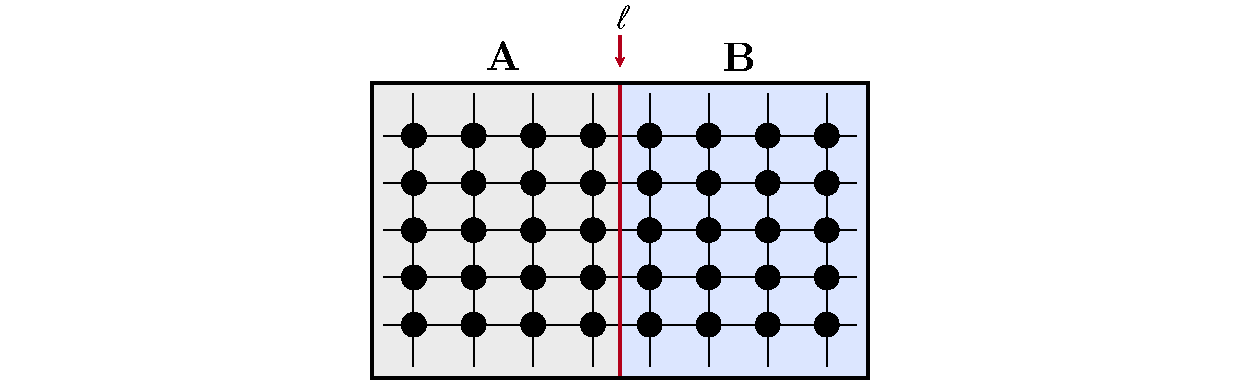
\includegraphics[width=\textwidth]{tci_eebipart.pdf}
\caption[Spatial bipartition]{Spatial bipartition of a system $\mathcal{S}$ into two (not necessarily identical) parts, $A$ and $B$. The length between two subsystems is denoted by $\ell$.}
\label{fig:spatial_bipart}
\end{figure}

For any vector $\ket{\Psi}$ representing a global state, there exists an orthonormal basis $\lbrace \ket{a_i} \rbrace$ (resp. $\lbrace \ket{b_j} \rbrace$) of $\mathcal{H}_{A}$ (resp. $\mathcal{H}_{B}$), such that $\ket{\Psi}$ may be rewritten using the Schmidt decomposition as
\begin{equation}
\ket{\Psi} = \sum^M_{m} \sqrt{\lambda_m} \ket{a_m} \otimes \ket{b_m}, \hspace*{1cm} \sum^M_{m} \lambda_m = 1,
\label{eq:schmidt_dec}
\end{equation}
where $\lambda_m \in [0, 1]$ are Schmidt coefficients and $M$ is the Schmidt rank (also called bond dimension), $M \leq \min (\mathrm{dim} \, \mathcal{H}_{A}, \mathrm{dim} \, \mathcal{H}_{B})$, defined as the number of non-zero coefficients $\lambda_m$. Such decomposition provides a straightforward criterion for separability; $M = 1$ tells that the state is the product state and can be factorized into a tensor product of state vectors in $\mathcal{H}_{A}$ and $\mathcal{H}_{B}$, $\ket{\Psi} = \ket{\psi_A} \otimes \ket{\psi_B}$, otherwise (when $M > 1$) the state is entangled. The von Neumann entanglement entropy in Eq.~\eqref{eq:vnee} can be expressed in terms of the Schmidt coefficients $\lambda_m$
\begin{equation}
S (\rho_A) = - \sum_m \lambda_m \log \lambda_m.
\end{equation}

\subsubsection{Area law}
For a $d$-dimensional system described by a gapped, local Hamiltonian with a finite correlation length, the entanglement entropy of the ground state typically follows~\cite{RevModPhys.82.277}
\begin{equation}
S (A) \simeq \alpha  \ell^{d -1 }
\label{eq:area_law}
\end{equation}
with $A$ a region of linear dimension $\ell$ with a smooth boundary and $\alpha$ a non-universal constant, which arises from a short-distance physics and strictly depends on the local properties of the system. This indicates that the EE is proportional to the area of the boundary between two subsystems, which is in contrast to generic excited states obeying volume-like scaling. The original motivation for studying area-like entropy scaling originally appeared in the context of black hole physics, where the Bekenstein-Hawking entropy turned out to be proportional to the surface area of the event horizon~\cite{PhysRevD.7.2333}. More importantly, the area law underlies the success of renormalization methods for many-body systems, because it determines which states are relevant in the low-energy sector - states scaling according to the area law belong to a tiny corner of the overall huge Hilbert space and focusing only on the sub-manifold of states significantly reduces the complexity of the problem. The validity of the area law was rigorously proven in several cases, including 1D gapped chains~\cite{Hastings_2007} or discrete versions of real free Klein-Gordon fields~\cite{PhysRevLett.94.060503}.

The situation becomes quite different in systems at criticality. For instance, one-dimensional chains at critical points exhibit conformal invariance and therefore may be described by conformal field theories (CFTs)\footnote{Conformal field theories are invariant under the action of the conformal group, which is the subgroup of coordinate transformations preserving angles and the background metric up to a scale factor.}. They then violate the area-like scaling with additional logarithmic corrections. In particular, if PBC are assumed and a subsystem $A$ has a length $x_A$, the vNEE in the thermodynamic limit scales like
\begin{equation}
S (A) \sim \frac{c}{3} \log x_A, 
\label{eq:area_law_log}
\end{equation}
with $c$ being the central charge of the corresponding CFT and, in an intuitive picture, counts the number of degrees of freedom\footnote{$c$ may not be an integer. For example, $c$ of a free-bosonic system is 1, while the critical Ising model has $c = 1/2$.}. The central charge defines the general class of phase transitions and depends only on the low-energy physics of a model, hence it may be used to detect a (topological) phase transition. Away from a critical point, where the correlation length $l$ is large but finite, the scaling of vNEE takes the form
\begin{equation}
S (A) \sim \frac{c}{3} \log l.
\label{eq:area_law_log_finite}
\end{equation}
For $x_A \rightarrow \infty$, it therefore saturates to a finite value. Similar logarithmic violation of the area law occurs also for free fermions in $d$-dimensions with a Fermi surface~\cite{PhysRevLett.96.010404, PhysRevLett.96.100503,PhysRevLett.105.050502}.
\subsubsection{Topological entanglement entropy}
As a comment, we would like to point an important observation that was made for systems with intrinsic topological order. In 2D, the vNEE has an additional subleading term $\gamma$ in the area law~\cite{RevModPhys.82.277}
\begin{equation}
S (A) = \alpha \ell - \gamma + \mathcal{O} \left( \frac{1}{\ell} \right)
\label{eq:TEE}
\end{equation}
where $ \mathcal{O} \left( 1 / \ell \right)$ represents terms vanishing in the limit $\ell \rightarrow \infty$. Global features of the entanglement are encoded in a universal term $ - \gamma$, known as topological entanglement entropy (TEE)~\cite{PhysRevLett.96.110404, PhysRevLett.96.110405}. TEE is directly related to the total quantum dimension $\mathcal{D}$, $\gamma = \log \mathcal{D}$, which characterizes anyonic quasiparticle excitations
\begin{equation}
\mathcal{D} = \sqrt{\sum_{\mu} \,  d_{\mu}^2},
\label{eq:quantum_dim}
\end{equation}
where the sum is over all types of quasiparticles $\mu$ with quantum dimension $d_{\mu}$. Abelian anyons have $ d_{\mu} = 1$, while non-Abelian anyons $d_{\mu} > 1$; however, obtaining an exact number is more complicated and requires to the knowledge of fusion rules between individual anyons~\cite{fradkin2013field}. Extracting $\gamma$ term heavily depends on the scaling analysis, which is not practical in numerical calculations~\cite{L_uchli_2010, PhysRevB.75.214407, PhysRevLett.98.060401}, and the knowledge of $\gamma$ is not sufficient to fully characterize a topologically ordered phase.

\subsection{Entanglement spectrum}
Entanglement entropy quantifies the correlations between two subsystems, but even more information can be extracted from the full spectrum of the density matrix $\rho_A$. In Ref.~\cite{PhysRevLett.101.010504}, Li and Haldane introduced the concept of entanglement spectrum to describe FQH systems, which has become a standard tool for studying topological systems, including topological insulators and superconductors~\cite{Fid:ES} or quantum spin chains~\cite{PhysRevLett.109.237208}. A core idea is to represent the Hermitian ($\rho_A = \rho_A^{\dagger}$) and positive semidefinite ($\braket{\phi | \rho_A| \phi} \geq 0, \all \ket{\phi} \in \mathcal{H}_A$) matrix $\rho_A$ in the form of a thermal density matrix
\begin{equation}
\rho_A = \frac{1}{Z} \, e^{- \beta^* H_A}
\label{eq:ent_spec}
\end{equation}
with the partition function $Z = \mathrm{Tr} \exp (-\beta^* H_{A})$ by convention taken to be one as it only shifts the energy, and the effective inverse temperature $\beta^* = 1/T$ set to $1$. $H_A$ is the so-called entanglement Hamiltonian and the ES refers to the eigenvalues $\varepsilon_m$ of $H_A$. Then, the entanglement spectrum is the logarithm of the eigenvalues of $\rho_A$
\begin{equation}
\varepsilon_m = - \ln \lambda_m.
\label{eq:loges}
\end{equation}
Summing over the ES results in the vNEE for a given subsystem. Remarkably, the low-energy edge spectrum of the physical Hamiltonian corresponds to the low-lying spectrum of the entanglement Hamiltonian $H_A$~\cite{PhysRevLett.101.010504, PhysRevB.84.205136} as dividing the system into two parts creates artificial boundaries\footnote{In special cases, this may not be true and the entanglement Hamiltonian falsely indicates a quantum phase transition, even if the physical system remains unchanged, see Ref.~\cite{Sondhi:univ}.}. This indicates that the ES is related to the bulk topology in analogy to the bulk-boundary correspondence.

\subsection{Free-fermionic systems}
In non-interacting fermionic systems, \ie, systems that are described by Hamiltonians billinear in fermionic creation and annihilation operators, the entanglement spectrum can be directly computed from the one-body correlation matrix restricted to the subsystem~\cite{Peschel}. Indeed, all higher-order correlation functions can be expressed in terms of two-point correlation functions due to Wick's theorem, and therefore the correlation matrix fully characterizes the system. For example, a four-point correlation function can be written as
\begin{equation}
\langle c_m^{\dagger} c_n^{\dagger} c_k c_l \rangle = \braket{c_m^{\dagger} c_l}  \braket{c_n^{\dagger} c_k} - \braket{c_m^{\dagger} c_k}  \braket{c_n^{\dagger} c_l} 
\end{equation}
or, in general, a $n$-point correlation function reads
\begin{equation}
\langle c_{i_1}^{\dagger} \ldots  c_{i_n}^{\dagger}  c_{j_1} \ldots c_{j_n} \rangle = (-1)^{n-1} \sum_{\sigma \in \mathbb{S}_n} (-1)^{P ( \sigma) } \braket{c_{i_1}^{\dagger} c_{j_{\sigma (1)}}} \ldots \braket{c_{i_n}^{\dagger} c_{j_{\sigma (n)}}}
\end{equation}
with the sum carries over the space $\mathbb{S}_n$ of the permutations $\sigma$ of $\lbrace 1 , \ldots, n \rbrace$ and $P(\sigma)$ is the sign of the permutation $\sigma$. Let $H$ be the bilinear Hamiltonian in the most general form, $H =  \sum_{ij} t_{ij} c_i^{\dagger} c_j$, and $C$ be the two-point correlation matrix 
\begin{equation}
C_{ij} = \langle c_i^{\dagger} c_j \rangle = \braket{\psi | c_i^{\dagger} c_j  | \psi},
\label{eq:corr_mat}
\end{equation}
where $i, \, j$ indices label lattice sites and $\ket{\psi}$ is an eigenstate of $H$ (Slater determinant). From now, consider only the subsystem $A$, so that $i, \, j$ indices are restricted to the $A$ part. We can rewrite $C_{ij}$ from Eq.~\eqref{eq:corr_mat} using the Gaussian density matrix $\rho_A \sim \exp ( - H_A )$, $C_{ij} = \langle c_i^{\dagger} c_j \rangle = \mathrm{Tr} \left( \rho_A  c_i^{\dagger} c_j \right)$, where $H_A$ is the entanglement Hamiltonian. Assuming $H_A$ to be also quadratic (as a consequence of Wick's theorem), the trace can be easily computed by transforming $H_A$ to the diagonal basis\footnote{Given a symmetric, positive matrix A, the trace of the matrix function $f(A)$ can be computed using the property $\mathrm{Tr} \left[ f(A) \right] = \sum_{i = 1}^n f(\lambda_i)$, where $\lambda_i, i = 1, \ldots, n$ are the eigenvalues of $A$.}, $H_A = \sum_l \varepsilon_l a_l^{\dagger} a_l$, where $\varepsilon_l$ are the corresponding single-particle eigenvalues and $\rho_A \sim \exp \left( - \sum_l \varepsilon_l a_l^{\dagger} a_l \right)$. From there, we arrive at the relation 
\begin{equation}
C = \frac{1}{1 + e^{\, H_A }}  \hspace*{0.5cm} \mathrm{or} \hspace*{0.5cm} H_A  = \ln \left[ \frac{1 - C}{C} \right].
\end{equation}
If we denote $\lbrace \zeta_l \rbrace$ the eigenvalues of the correlation matrix $C$, we see a one-to-one correspondence between the eigenvalues of $C$ and $H_A$
\begin{equation}
\zeta_l = \frac{1}{1+e^{\varepsilon_l}}.
\end{equation}
For periodic systems, where the momenta $\mathbf{k}$ remain good quantum numbers, the Hamiltonian $H$ can be written in reciprocal space with the many-body ground state being a Fermi sea
\begin{equation}
\ket{GS} = \prod_{\mathbf{k} n}  a^{\dagger}_{\mathbf{k} n} \ket{0}
\end{equation}
with operators $a^{\dagger}_{\mathbf{k} n}$ corresponding to creation a particle with the momentum $\mathbf{k}$ and $n$ running over the occupied single-particle Bloch states. Suppose we have a 2D system, where the spatial bipartition in position space is performed along a one chosen direction. Then, the translational symmetry is broken in a direction orthogonal to the cut, but the momentum $k$ parallel to the cut can be still used to label the eigenstates of the system. Therefore, it is possible to evaluate the correlation matrix for each $k$-point separately. Such $k$-dependent $C$ matrix is Hermitian and can be regarded as a spectrally flattened physical Hamiltonian with the eigenvalues $\zeta_k \in [0, 1]$. Most of the eigenvalues in the spectrum of $C_{ij}(k)$ lie exponentially close to either 1 or 0, depending whether the bulk states are fully localized in the subsystem $A$ or $B$, respectively, and do not contribute to the entanglement entropy. However, the states crossing the partition boundary give rise to the non-zero EE. If the system is in a topological phase, $C_{ij} (k)$ will reveal the spectral flow associated with a continuous set of intermediate eigenvalues \cite{Hughes:inv, Vish:inv}. From now, we refer to the eigenvalues of the correlation matrix as the single-particle entanglement spectrum, which is a conventional practice in the literature \cite{Alex:CM, Vish:inv, Hughes:inv}. Having the correlation matrix $C_{ij}$ restricted to subsystem $A$, the entanglement entropy can be calculated by summing all eigenvalues of $C$
\begin{equation}
S(A) \equiv S_A = - \sum_a \left[ \zeta_a \log \zeta_a + \left( 1 - \zeta_a \right) \log \left( 1 - \zeta_a \right) \right].
\label{eq:entCij}
\end{equation}
We see that the contribution to $S_A$ arises from the intermediate values of $\zeta_a$; if $\zeta_a = 0$ or $\zeta_a = 1$, then $S_A$ vanishes. In a case of the $k$-resolved correlation matrix, $S_A$ is obtained by summing over the $S_A (k)$ at each $k$-momenta with a normalization factor being the total number of unit cells in the system~\cite{Ryu:EE}.

\section{Bismuth and antimony monolayers}
\label{sec:bismuth-antimony}
Several topological aspects of bismuth and antimony-based systems have been investigated in the past. Elemental 3D Bi and Sb share the same rhomohedral R$\bar{3}$m crystal structure, which can be viewed as a set of stacked hexagonal atomic layers along the (111) crystallographic direction with the interlayer interaction much weaker than the interactions within each layer. The bulk systems are semimetals with a direct energy gap over the BZ, but a negative indirect gap due to band overlap. Remarkably, Bi$_{1-x}$Sb$_{x}$ alloy was the first experimentally confirmed topological insulator, where doping bulk Bi with Sb atoms leads to a band inversion around $x \sim 0.04$ and then to a topological phase observed in a range of $0.07 < x <  0.22$. Protected surface states were confirmed experimentally with ARPES~\cite{Hsieh2008}, spin-resolved ARPES~\cite{Hsieh919} and scanning tunneling microscope (STM)~\cite{Roushan2009} and are in an agreement with theoretical calculations~\cite{PhysRevB.78.045426, PhysRevB.80.085307}. 
With a decreasing thickness, these systems undergo a semimetal-semiconductor transition as quantum confinement plays substantial role~\cite{stable:bi111}. A single layer of bismuth was predicted to host quantum spin Hall states~\cite{Murakami:BiQSH}, which was later on confirmed by the observation of one-dimensional protected edge modes using STM~\cite{drozdov, kawakami2015one, spatialandenergy}. With a refined topological classification, bulk bismuth was also established as a higher-order topological insulator with conducting 1D hinge channels~\cite{Schindler2018}. Moreover, protected one-dimensional edge states were detected in Bi$_2$Se$_3$ thin films \cite{BiSe2d, Zhang:1} and at an interface between heterostructures Bi(111)/Bi$_2$Te$_3$ \cite{BiTe3inter}. Antimony films with less than four layers are expected to be topologically trivial~\cite{Sb:triv}. To induce a transition between trivial and QSH insulating phases, appropriate structure modifications were proposed, including strain~\cite{jin2015quantum, Sb:nontriv} or a perpendicular electric field applied to an already strained layer~\cite{wang2014topological}. 

\begin{figure}[H]
\centering
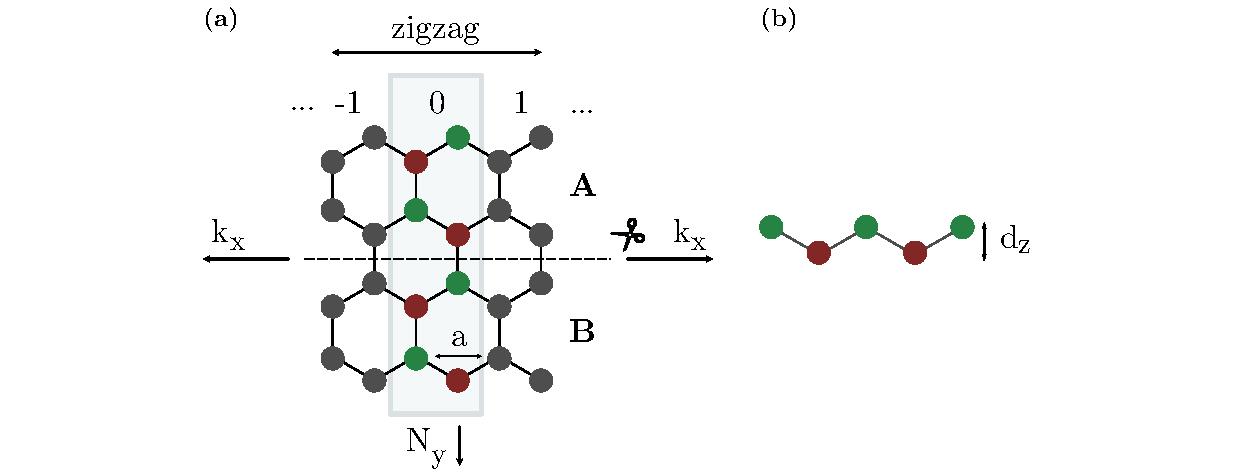
\includegraphics[width=0.95\textwidth]{tci_honeybipart.pdf}
\caption[Lattice structure of Bi and Sb monolayers]{A schematic representation of bismuth and antimony monolayers. \textbf{(a)} top and  \textbf{(b)} side views of a honeycomb lattice in a ribbon geometry with a zigzag edge termination and a layer thickness $d_z$. We investigate a finite strip with $N_y$ unit cells consisting of four atoms and periodicity in $x$-direction, hence $k_x$ is a good quantum number. Sites belonging to different sublattices forming a honeycomb lattice are distinguished by red and green colors. We divide system into two parts, $A$ and $B$, with a cut performed in the middle of a ribbon denoted by a dashed line to compute the entanglement measures.}
\label{fig:bisb_latt}
\end{figure}

Free-standing monolayers of bismuth and antimony(111)\footnote{The term \emph{bilayer} is sometimes used to indicate that a monolayer consists of atoms forming two spatially separated sublattices.} have a honeycomb lattice structure (such arrangement is often called a $\beta$-allotrope) as depicted in Fig.~\ref{fig:bisb_latt}. A primitive unit cell contains two atoms, however a conventional hexagonal unit cell explicitly shows three-fold rotation $C_3$ and inversion $\mathcal{I}$ symmetries present in the systems. To describe the electronic properties, we use $sp^3$ tight-binding model developed in Ref.~\cite{Liu:Allen} for bulk bismuth and antimony, neglecting hoppings between monolayers as proposed in Ref. \cite{Murakami:BiQSH}. Interatomic hoppings up to the next-nearest neighbors and atomic spin-orbit coupling term $\lambda \mathbf{L}\cdot\mathbf{S}$ are parametrized within the Slater-Koster approach~\cite{Slater:Koster}. The Hamiltonian of the model is a $16 \times 16$ matrix ($4$ orbitals $\times$ $2$ atoms per unit cell $\times$ spin) and reads
\begin{equation}
\begin{aligned}
H &= \sum_{\alpha, \sigma, R} \ket{\alpha ,\sigma ,R}  E_\alpha   \bra{\alpha ,\sigma ,R}  + \sum_{\alpha ,\beta ,\sigma ,R, R'}  \ket{\alpha ,\sigma ,R}  V_{\alpha \beta }'   \bra{\beta ,\sigma ,R'} +  \\
&\sum_{\alpha ,\beta ,\sigma ,R,R''} \ket{\alpha ,\sigma ,R}  V_{\alpha \beta} ''     \bra{\beta ,\sigma ,R''} +  \frac{\lambda}{3} \sum_{\alpha ,\sigma ,\sigma ',R} \ket{\alpha ,\sigma ,R} \mathbf{L} \cdot \mathbf{S}  \bra{\alpha ,\sigma ',R}  + \mathrm{h. c}, 
\end{aligned}
\label{eq:liu allen}
\end{equation}
$\alpha, \beta = \lbrace s, p_x, p_y, p_z \rbrace$ label the orbitals and $\sigma, \, \sigma ' = \lbrace \uparrow, \, \downarrow \rbrace $ denote the spin degrees of freedom. $E_{\alpha}$ are the on-site energies, $V_{\alpha \beta}$ correspond to Slater-Koster two-center integrals between ${\alpha}$ and ${\beta}$ orbitals, and $R$ are the atomic positions (with $R'$ being NN atom and $R''$ -- NNN atom). The last term describes the spin-orbit coupling (SOC) with strength $\lambda$. According to Ref.~\cite{Chadi}, $1/3$ factor is introduced to the renormalized atomic SOC in order to obtain correct SOC splitting of the valence band. All model parameters are listed in Table~\ref{tab:TB}. Most of them differ by less than $15\%$ between bismuth and antimony crystals, but a stark difference appears in the SOC constant $\lambda$ being $2.5$ times larger in bismuth.

\begin{table}[H]
\centering
\begin{tabular}{|c|c|c||c|c|c|}
\hline 
Parameter (eV) & Bi & Sb & Parameter (eV)  & Bi & Sb \\ \hline
E$_{s}$ & -10.906 & -10.068 & V'$_{sp\sigma}$ & 0.433 & 0.478 \\ 
E$_{p}$ & -0.486 & -0.926 & V'$_{pp\sigma}$  & 1.396 & 1.418  \\
V$_{ss\pi}$ & -0.608 & -0.694 & V$'_{pp\pi}$ & -0.344 & -0.393 \\
V$_{sp\sigma}$ & 1.320 & 1.554 & V''$_{ss\sigma}$ & 0 & 0 \\
V$_{pp\sigma}$ & 1.854 & 2.342 & V''$_{sp\sigma}$ & 0 & 0\\
V$_{pp\pi}$& -0.600 & -0.582 & V''$_{pp\sigma}$ & 0.156 & 0.352 \\
V'$_{ss\sigma}$& -0.384 & -0.366 & V''$_{pp\pi}$ & 0 & 0\\
$\lambda$ & 1.5 & 0.6 &   & & \\
\hline
a ($\textnormal{\AA}$) & 4.53 & 4.30 & $d_z$ ($\textnormal{\AA}$) & 1.58$^{*}$ & 1.64$^{**}$ \\
d$_1$ ($\textnormal{\AA}$) & 3.062 & 2.902 &  &  &\\
\hline
\end{tabular} 
\caption[Tight-binding parameters for bismuth and antimony taken]{Tight-binding parameters for bismuth and antimony taken from Refs.~\cite{Liu:Allen}, \cite{stable:bi111}$^*$, \cite{Sb:nontriv}$^{**}$. $d_1$ denotes nearest-neighbor distance between sites in a honeycomb lattice.}
\label{tab:TB}
\end{table}

In band insulators, the SOC plays a fundamental role in topological phase transitions and is associated with a band inversion -- states of different symmetries are inverted at the conduction band minimum (CBM) and valence band maximum (VBM). The band inversion can occur between orbitals with different parities, for example between even $s$-orbitals and odd $p$-orbitals (which was observed, for instance, in HgTe/CdTe quantum wells~\cite{MolenkampQSHE2007}) or between different $p$ orbitals (as in 3D TIs with a single Dirac cone on the surface: Bi$_2$Se$_3$, Bi$_2$Te$_3$ and Sb$_2$Te$_3$~\cite{Zhang2009}). SOC effect is in particular noticeable in the materials containing heavy elements as SOC strength scales like $Z^4$ with $Z$ being the atomic number. A further enhancement of the energy gap opening by SOC is possible by including additional effects such as electron-electron correlations, which leads to the band inversion between $d$ and $f$ orbitals; on that note, an idea of topological Kondo insulators with SmB$_6$ as a material example was introduced~\cite{doi:10.1146/annurev-conmatphys-031214-014749}. One way to quantify the SOC-driven band inversion is based on the so-called spin-orbit spillage, which measures the degree of mismatch between the occupied band projection operators with and without SOC~\cite{SOCspillage}.

In Fig.~\ref{fig:bs_bisb}, we present the orbital-projected band structures for buckled bismuth and antimony single layers along the high-symmetry path K-$ \Gamma$-M-K in the first BZ. Lowest energy bands are composed mostly of $s$-orbitals and are separated by a large gap from $p$-type bands close to the Fermi level. Bi monolayer has an indirect energy gap around $\Gamma$ with $E_{gap} \sim 0.4$ eV, while Sb layer is a direct gap semiconductor with $E_{gap} \sim 1.3$.

\begin{figure}[H]
\centering
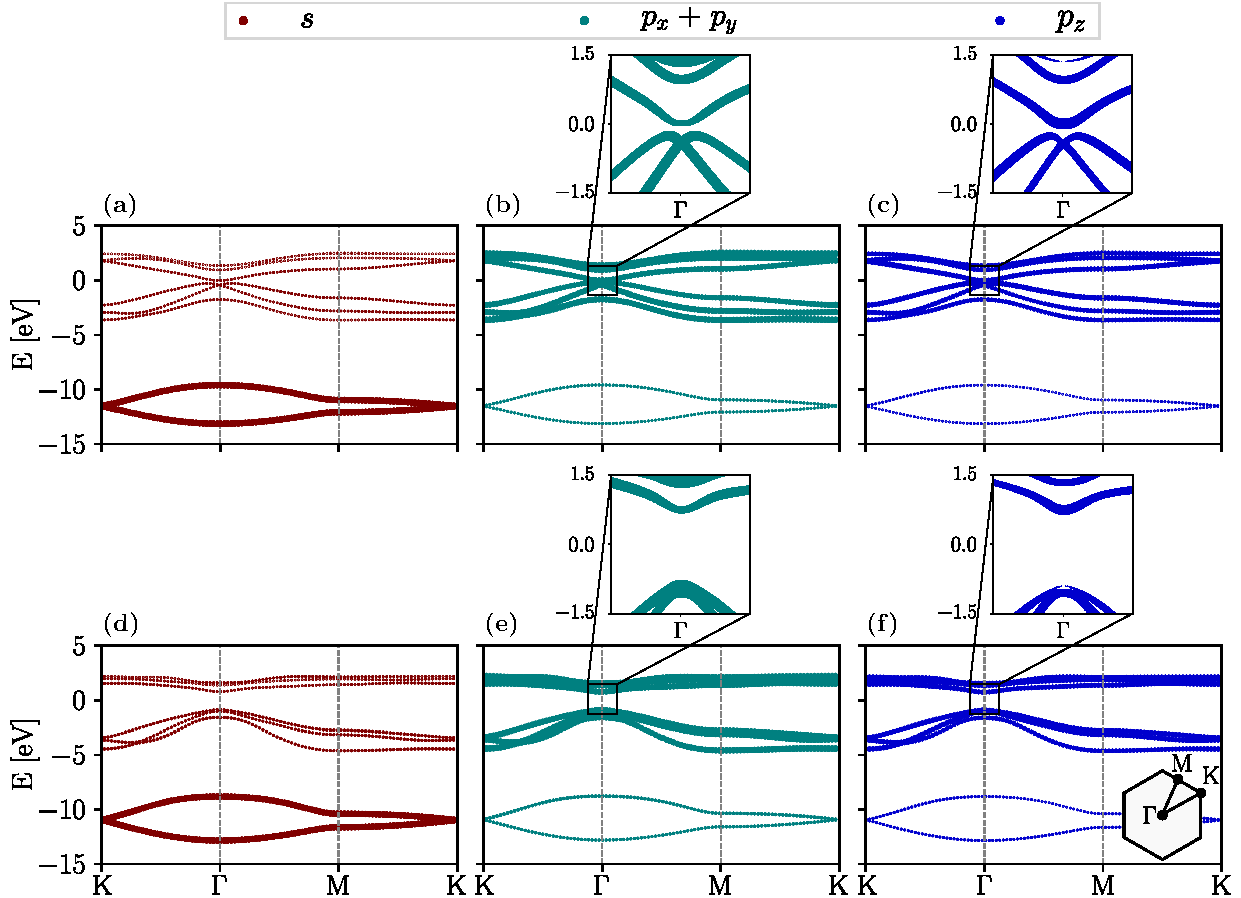
\includegraphics[width=\textwidth]{tci_bandstructures.pdf}
\caption[Band structures of bismuth and antimony monolayers]{Band structures of infinite \textbf{(a, b, c)} bismuth and \textbf{(d, e, f)} antimony along the high-symmetry path K-$ \Gamma$-M-K. Red, teal and blue colors correspond to the orbital contribution of $s$, in-plane $p_x + p_y$ and out-of-plane $p_z$ orbitals, respectively, with the circle radius denoting the weight of the contribution. Low-energy bands have $s$-type character, while the bands close to the Fermi level are $p$-type. Both materials have a well-defined band gap around $\Gamma$-point. For a Bi layer, the conduction band minimum has $p_z$ character, while the valence band maximum is $p_x + p_y$ mixture. In a case of Sb single layer, all $p$ orbitals contribute to the conduction band, but the valence band retains $p_x + p_y$-like.}
\label{fig:bs_bisb}
\end{figure}

\subsection{Edge states in a ribbon geometry}
Equipped with useful formulations of entanglement measures for non-interacting systems, we now move to study topological properties of nanoribbons with periodicity in $x$ direction and a zigzag edge termination\footnote{Armchair ribbons posses an extra pair of edge states in a gap, which leads to spurious modes in the ES. As we investigate topological properties inherited from a bulk, not an edge termination, the conclusions would hold for both types of edges.}, depicted in Fig.~\ref{fig:bisb_latt}. We set the width of the strip $N_y = 6$, which corresponds to $N_{\mathrm{at}} = 48$ atoms in the systems. This system size ensures that two opposite edges are sufficiently far, so no hybridization between edge states is expected and the spatial cut into two parts performed exactly in the middle of ribbons guarantees that the edge modes are perfectly confined within the subsystems. In Fig.~\ref{fig:ribbon}, we compare the results for buckled bismuth and antimony. Edge states spectrally connecting the conduction and valence bands are observed for the Bi monolayer, which translates into the presence of spectral flow in the ES, see Fig.~\ref{fig:ribbon}~(a) and (b). It is in contrast with the pure Sb structure, where almost flat dangling bonds are exhibited in the energy gap, but they are not associated with non-trivial bulk topology (consult Fig.~\ref{fig:ribbon}~(d) and (e)). We note that mid-gap states with $\zeta = 0.5$ in the ES are related to the inversion symmetry present in the system. 

\begin{figure}[H]
\centering
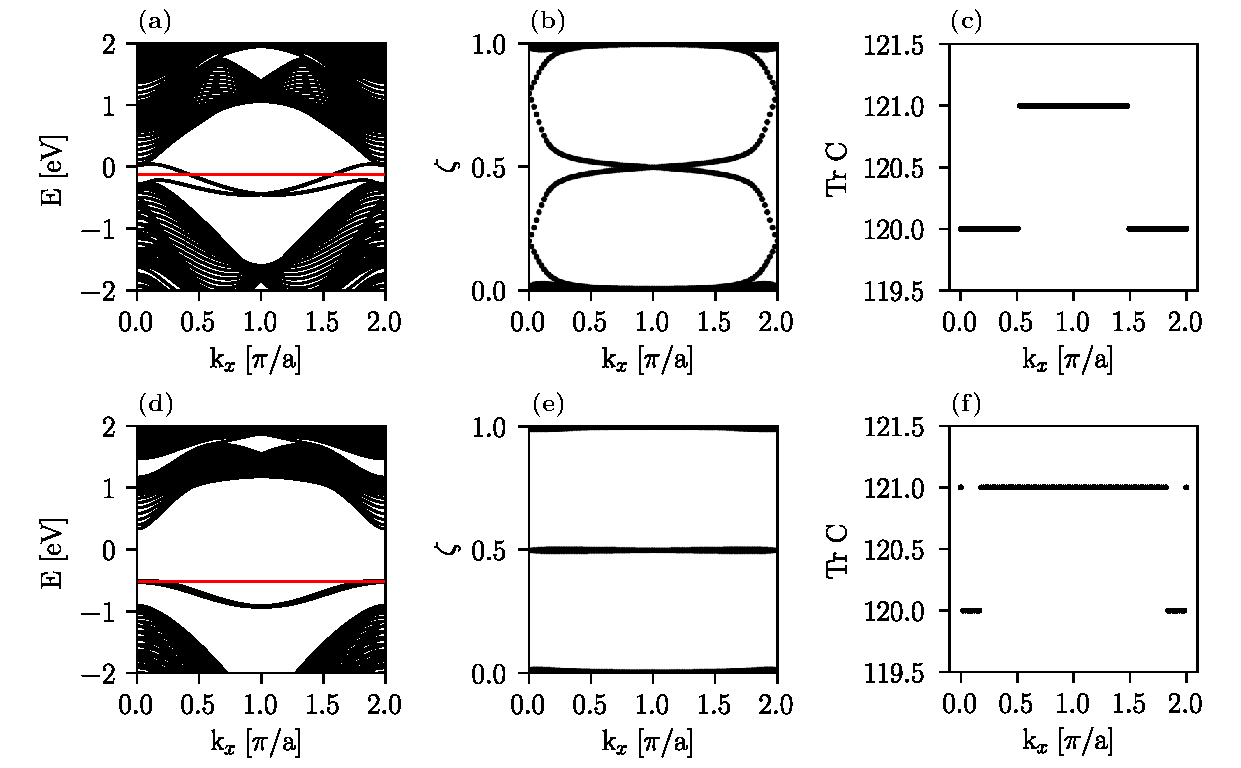
\includegraphics[width=\textwidth]{tci_es_ribbon.pdf}
\caption[Energy and entanglement spectra, together with a trace index for bismuth and antimony monolayers]{Energy and entanglement spectra, together with a trace index for \textbf{(a, b, c)} bismuth and \textbf{(d, e, f)} antimony monolayers. Non-trivial topological nature of Bi layer is manifested by a pair of edge modes connecting the conduction and valence bands, as well in the presence of a spectral flow in the entanglement spectrum and a single discontinuity in trace index in the half of BZ at $k_x = \pi / 2$. In contrast, flat bands located in the gap in the energy spectrum of Sb layer are trivial, which is reflected by an even number of discontinuities in the trace index.}
\label{fig:ribbon}
\end{figure}

In a semi-infinite geometry, the trace of the correlation matrix describing a subsystem, $\mathrm{Tr} (C)$, called trace index allows to easily distinguish whether the system is in a topological or a trivial phase by counting the number of discontinuities in the trace index. Physical edge states in the bulk gap that cross the Fermi level lead to discontinuities in $\mathrm{Tr} (C)$. For the systems in AII symmetry class, zero (non-zero) $\mathbb{Z}_2$ index corresponds to even (odd) number of discontinuities mod 2 in the half of BZ~\cite{Hughes:inv}. 

\subsection{Topological phase transitions}
Furthermore, we demonstrate the behavior of $S_A$ defined in Eq.~\eqref{eq:entCij} across different topological phase transitions (TPTs). To avoid boundary effects, we apply periodic boundary conditions to the ribbon also in the $y$ direction. As the system is now effectively a torus, dividing it into two spatial parts introduces two boundaries and results in a spectral symmetry with all the ES eigenvalues coming in pairs \cite{Sondhi:univ}. We perform calculations for $N_y = 7, \, 10$ and $13$ unit cells, which corresponds to $N_{\mathrm{at}} = 28, \, 48, \, 52$ atoms in a stripe, respectively. 

\subsubsection{Composition-induced phase transition in Bi$_{1-x}$Sb$_x$}
We begin with the transition to a trivial phase driven by the antimony content in Bi$_{1-x}$Sb$_x$ alloy and treat it within a virtual crystal approximation. Instead of considering a supercell consisting of different number of bismuth and antimony atoms (which would be required to maintain translational invariance), we replace atoms in a unit cell by a pseudoatom that has properties being weighted averages over the properties of Bi and Sb. Thus, the values of hopping integrals between all lattice sites are effectively scaled with respect to $x$
\begin{equation}
t_x = (1-x) \cdot t_{\mathrm{Bi}} + x\cdot t_{\mathrm{Sb}},
\label{eq:VCA}
\end{equation}
where $t_{\mathrm{Bi/Sb}}$ are parameters from taken Table \ref{tab:TB}. A transition from QSH insulating phase to trivial insulator with increasing $x$ in Bi$_{1-x}$Sb$_x$ is related, in general, to a decreasing value of the spin-orbit coupling constant. 

\begin{figure}[H]
\centering
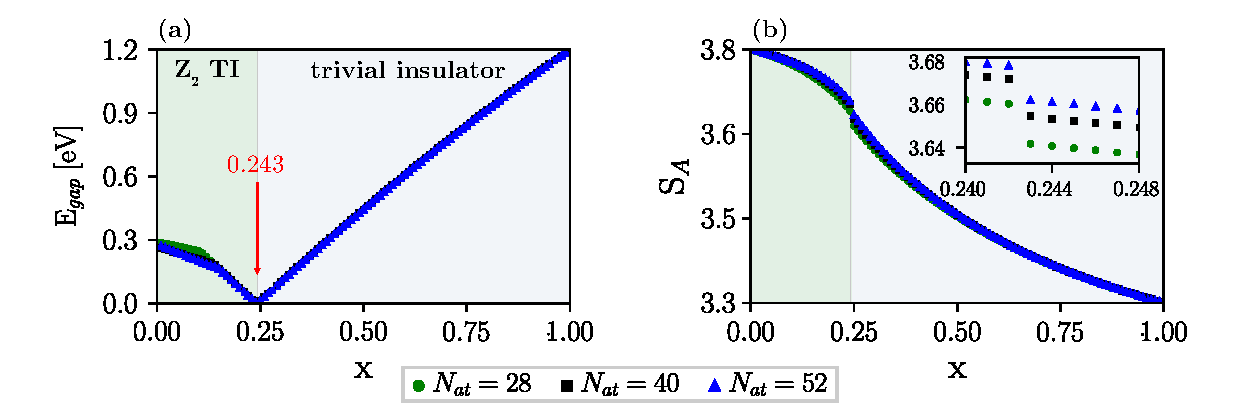
\includegraphics[width= 0.95\textwidth]{tci_TPT_composition.pdf}
\caption[Energy gap and entanglement entropy as a function of composition $x$ in free-standing Bi$_{1-x}$Sb$_x$]{\textbf{(a)} Energy gap and \textbf{(b)} entanglement entropy as a function of composition $x$ in a free-standing Bi$_{1-x}$Sb$_x$ layer. The transition from a $\mathbb{Z}_2$ topological insulator to a trivial insulator goes through a bulk gap closing point (indicated by a red arrow) at $ x = 24.3 \%$ antimony composition and is accompanied by a discontinuity in the scaling of entanglement entropy, regardless of system size (see inset).}
\label{fig:TPT_composition}
\end{figure}

In Fig.~\ref{fig:TPT_composition}~(a), we show the band gap scaling with respect to $x$. Finite-size effects are manifested as a kink in the energy gap evolution around $x\sim 0.12$ for a system with $N_{\mathrm{at}} = 28$ atoms. The energy gap of clean bismuth, $x = 0$, is $ E_{\mathrm{gap}} = 0.3$ eV and decreases as a function of $x$ up to the point $x = 0.243$, where the band gap closing occurs (this value is in an agreement with calculations done for infinite 2D crystal). A further change of antimony concentration leads to the topological phase transition into a trivial phase, with $E_{gap}$ increasing linearly to the value of $1.2$ eV for elemental antimony. The dependence of $S_A$ on the composition $x$ is illustrated in Fig.~\ref{fig:TPT_composition}~(b). Clean Bi layer is characterized by the largest value of the entanglement entropy which decreases monotonically with $x$ to its minimal value for pure Sb. A finite discontinuity of $S_A$ at $x = 0.243$ is observed for all investigated system sizes and coincides with the closing of the bulk gap.

\subsubsection{Electric field-driven transition in a bismuth layer}
External fields are convenient parameters that may be used for controlling band topology. Here, we show that a TI phase in a bismuth layer can be toggled off by applying a perpendicular electric field $E_{Field}$. The effect of $E_{Field}$ can be modelled by including an electrostatic energy difference $V_{Field}$ between the two sublattices. Due to the spatial separation $d_z$, atoms in the lattice are affected differently by the external field. Because the absolute values of the potentials on each sublattice does not matter, but only their difference, we can therefore capture the effect of $E_{Field}$ by adding potentials on two sublattices with opposite signs, $V^{R}_{Field} = - V^{G}_{Field}$, similar to a staggered potential. $R$ and $G$ refer to, respectively, the red and green sites in Fig.~\ref{fig:ribbon} belonging to different sublattices.
 
\begin{figure}[H]
\centering
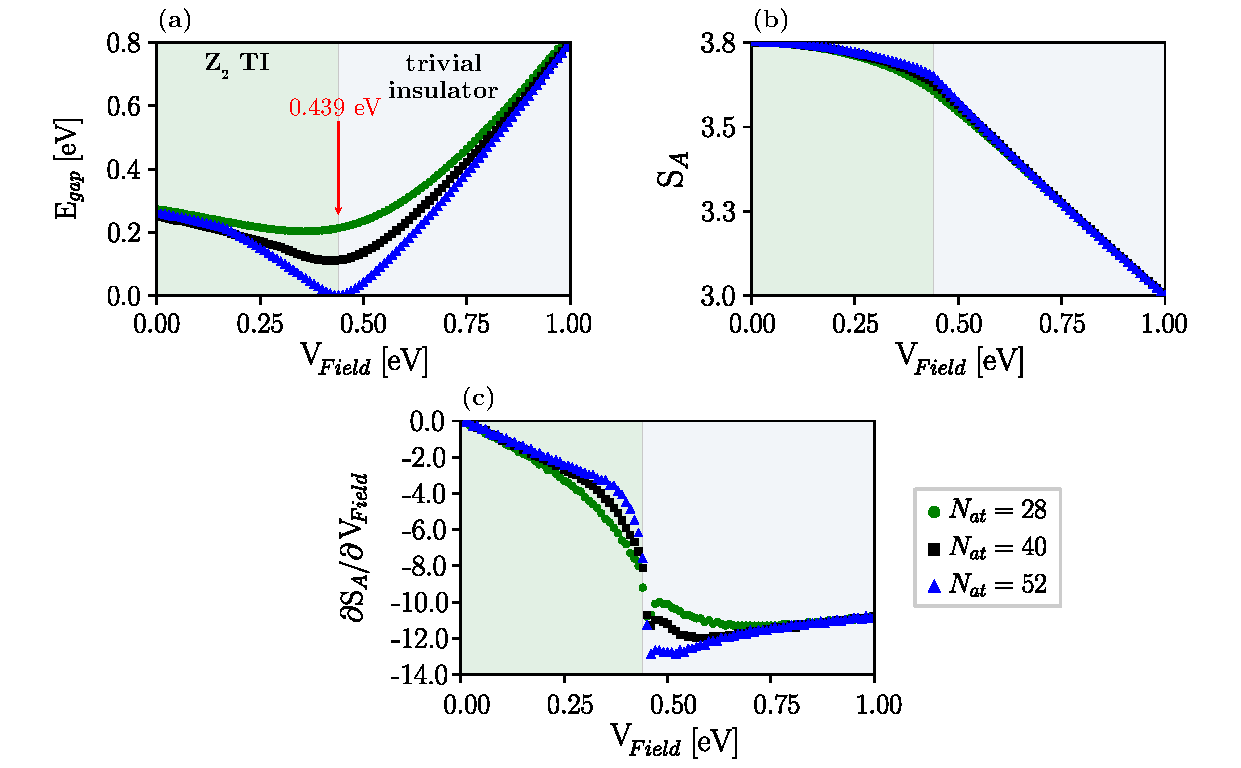
\includegraphics[width= 0.95\textwidth]{tci_TPT_efield.pdf}
\caption[Energy gap, entanglement entropy and its second derivative as a function of external potential due to electric field]{\textbf{(a)} Energy gap, \textbf{(b)} entanglement entropy and \textbf{(c)} its second derivative as a function of external potential $V_{Field}$ due to electric field. For a sufficiently wide system, the band gap closes at $V_{Field} = 0.439$ eV, which is indicated by a red arrow. Entanglement entropy remains a continuous function, while the derivative becomes discontinuous at band gap closing point.}
\label{fig:TPT_efield}
\end{figure}

The energy band gap as a function of the external potential $V_{Field}$ is plotted in Fig.~\ref{fig:TPT_efield}~(a). Firstly, we point out that the band gap does not close completely even for a wide system with 52 atoms, but in the limit of $N \rightarrow \infty$ we checked that it closes at $V_{Field} = 0.439$ eV. Interestingly, $S_A$ is sensitive to the bulk gap closing in finite systems, which is indicated by an inflection point in the scaling of entanglement entropy (consult Fig.~\ref{fig:TPT_efield}~(b)) and a corresponding discontinuity in the numerically obtained first derivative of $S_A$ with respect to $V_{Field}$, $\partial S_A / \partial V_{Field}$, in Fig.~\ref{fig:TPT_efield}~(c). This point is more visible for larger system sizes as the sharpness of the discontinuity  in the derivative is strongly size-dependent. In the large $V_{Field}$ limit, the energy scale given by the hopping integrals and the SOC is relatively negligible and the states are fully localized on the lattice sites. As a consequence, two sublattices become energetically disconnected and the entanglement entropy saturates to almost zero value and the ES spectrum consisting only of 0's and 1's. Moreover, the inversion symmetry is broken by a strong external perturbation, which is reflected in the single-particle entanglement spectrum. In Fig.~\ref{fig:ES_efield}, we show two spectra: before (at $V_{Field} = 0.24$ eV) and after ($V_{Field} = 0.54$ eV) the topological phase transition. The separated branches of states seen in Fig.~\ref{fig:ES_efield}~(b) are moving towards 0's and 1's eigenvalues by increasing $V_{Field}$. 

\begin{figure}[H]
\centering
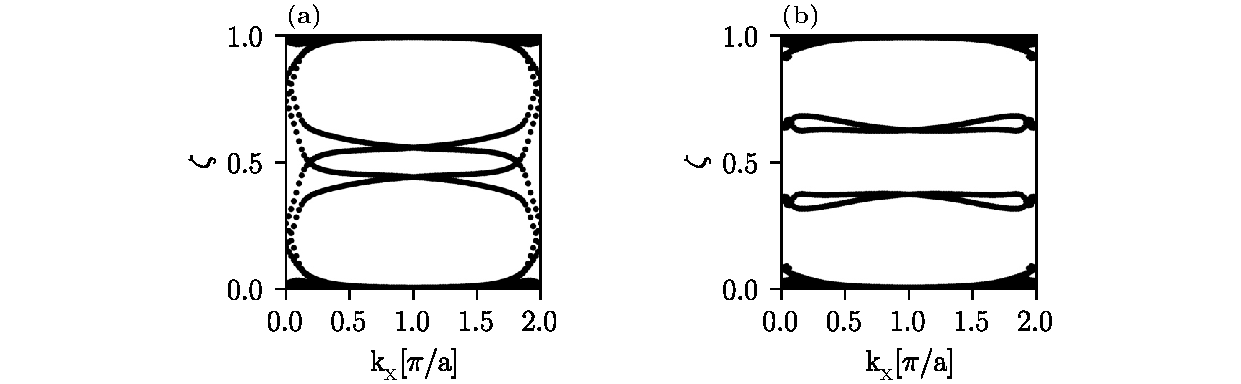
\includegraphics[width= 0.95\textwidth]{tci_efield_es.pdf}
\caption[Entanglement spectrum in a presence of electric field]{Entanglement spectrum \textbf{(a)} before and \textbf{(b)} after topological phase transition induced by an electric field. For large $V_{Field}$ values, the inversion symmetry is lost as states pinned to $\zeta = 0.5$ are not observed anymore.}
\label{fig:ES_efield}
\end{figure}

\subsubsection{Effect of strain on an antimony layer}
A free-standing monolayer of antimony is characterized by a vanishing $\mathbb{Z}_2$ invariant, but a TI phase can be induced by applying a tensile strain~\cite{Sb:nontriv}. We model this transition by scaling the hopping integrals due to the change of bond lengths and angles. Following Harrison \cite{harrison}, all hopping parameters in the model are then modified by a constant factor
\begin{equation}
V_{\alpha \beta } = V_{\alpha \beta}^0 \cdot \left( \frac{d}{d_0} \right)^{-n},
\label{eq:hopping_rescale}
\end{equation}
where $V_{\alpha \beta}^0$ are values taken from Table~\ref{tab:TB} corresponding to the unstrained case, while $d$ and $d_0$ are, respectively, new and unmodified bond lengths. Within this approach, no structural phase transitions are expected as all hopping terms are scaled by the same factor and the symmetries of the system are preserved. The band gap decreases monotonically with a strain up to a critical value of $13.8 \%$, when it closes, which we illustrate in Fig.~\ref{fig:TPT_strain}~(a). As in case of the composition-induced TPT, a small discontinuity in the entanglement entropy is also observed.

\begin{figure}[H]
\centering
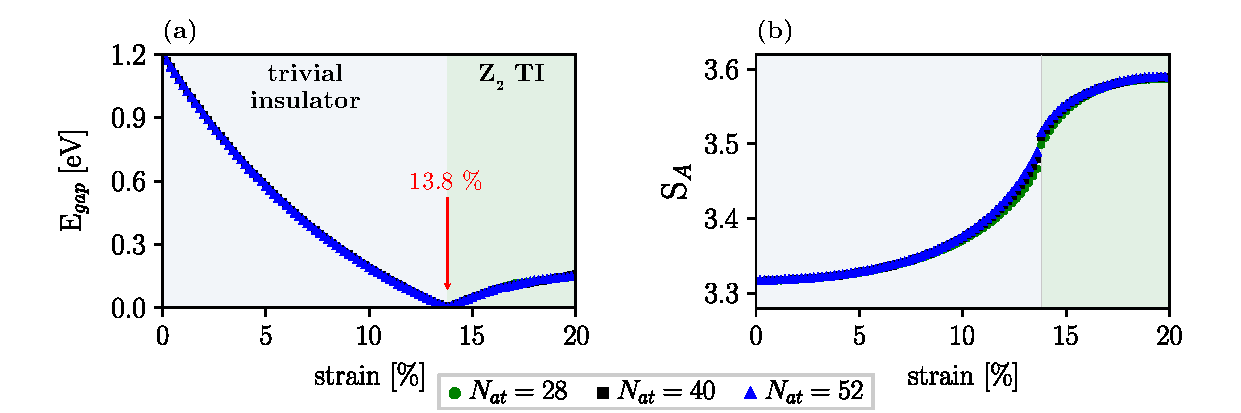
\includegraphics[width= 0.95\textwidth]{tci_TPT_strain.pdf}
\caption[Energy gap and entanglement entropy as a function of strain in free-standing antimony monolayer]{\textbf{(a)} Energy gap evolution and \textbf{(b)} entanglement entropy scaling with respect to strain. The band gap closes at $13.8 \%$ value of strain and occurs with a discontinuity of finite extend in entanglement entropy.}
\label{fig:TPT_strain}
\end{figure}


\section{Bismuthene and antimonene}
\label{sec:bismuthene-antimonene}
We now move to completely planar structures of bismuth and antimony called, in analogy to graphene, bismuthene and antimonene. Recent experimental works have reported a growth of bismuthene on silicon carbide SiC(0001)~\cite{Reis287}, after several failed attempts to synthesize hexagonal flat Bi on Si(111) substrate~\cite{KUZUMAKI20101044, Miwa_2003}. A successful synthesis of Bi on NbSe$_2$ led to a discovery of its novel allotrope in a form of compressively strained 2D triangular lattice~\cite{Fangeaaq0330}. Remarkably, stable free-standing bismuthene structures were realized as well~\cite{Yang2020}. With the experimentally measured bulk gap of 800 meV, bismuthene is amongst the most promising material candidates for a room temperature QSH effect~\cite{AsSbBiSiC1, AsSbBiSiC2}. As yet, there are not many experimental studies on the electronic properties of atomically thin Sb. Only recently, several reports demonstrated a successful fabrication of a monolayer structure of antimony~\cite{SbonAg, SbSyntMBA, SbonGe}, with a predicted energy gap of $47.7$ meV~\cite{SbonAg}.

To model flat monolayers, we set the buckling $d_z$ to zero and use the lattice constants determined from first-principle calculations~\cite{Hsu_2015} for bismuthene ($a = 5.35$ \AA) and antimonene ($a = 5.00$ \AA). At $d_z = 0$, both systems have the full six-fold rotational symmetry $C_6$ and, most importantly, the mirror symmetry under $z \rightarrow -z$, \ie, the mirror plane parallel to the $xy$ plane, is restored. $\mathcal{M}_z$ symmetry protects a TCI phase, which we firstly confirm by computing the mirror Chern number via the Kubo formula for each mirror sector~\cite{Hsu2016} 
\begin{equation}
\mathcal{C}_{\pm} = \frac{1}{2 \pi} \int_{BZ}   d k_x d k_y \sum_{\epsilon_n < E_F < \epsilon_m} 2 \, \mathrm{Im} \, \frac{\braket{u^{\pm}_{\mathbf{k} n} | \frac{\partial H}{\partial k_x}  |  u^{\pm}_{\mathbf{k} m}}    \braket{u^{\pm}_{\mathbf{k} m} | \frac{\partial H}{\partial k_y}  |  u^{\pm}_{\mathbf{k} n}}}{ (\epsilon_n - \epsilon_m)^2},
\label{eq:mirror-chern-num}
\end{equation}
where $E_F$ is the Fermi level, while $\epsilon_{n/m}$ are the eigenvalues associated with the eigenstates $\ket{u_{\mathbf{k} n/m}}$ of the Hamiltonian. The $\mathbb{Z}_2$ invariant vanishes for these planar systems, but we obtain non-zero $|\mathcal{C}_{\mathcal{M}}| = 2 $ (using Eq.~\eqref{eq:mirror_chern}), which is consistent with an even number of edge modes crossing the Fermi level in a ribbon geometry, see Fig.~\ref{fig:free-substrate-bisb}~(a, e). Therefore, we conclude that the boundary modes are solely protected by $\mathcal{M}_z$.

The different topological properties of buckled and planar monolayers are also reflected in the orbital composition of the bands around $E_F$. In Fig.~\ref{fig:bs-anti-bism}, we show the orbital-resolved band structures along the same K-$\Gamma$-M-K path for bismuthene and antimonene. In both cases, the valence bands are mostly composed of $p_z$ orbitals around the $K$ point, where an indirect gap is observed (with $E_{gap} \sim 0.6$ eV for bismuthene and $E_{gap} \sim 0.5$ eV for antimonene).

\begin{figure}[H]
\centering
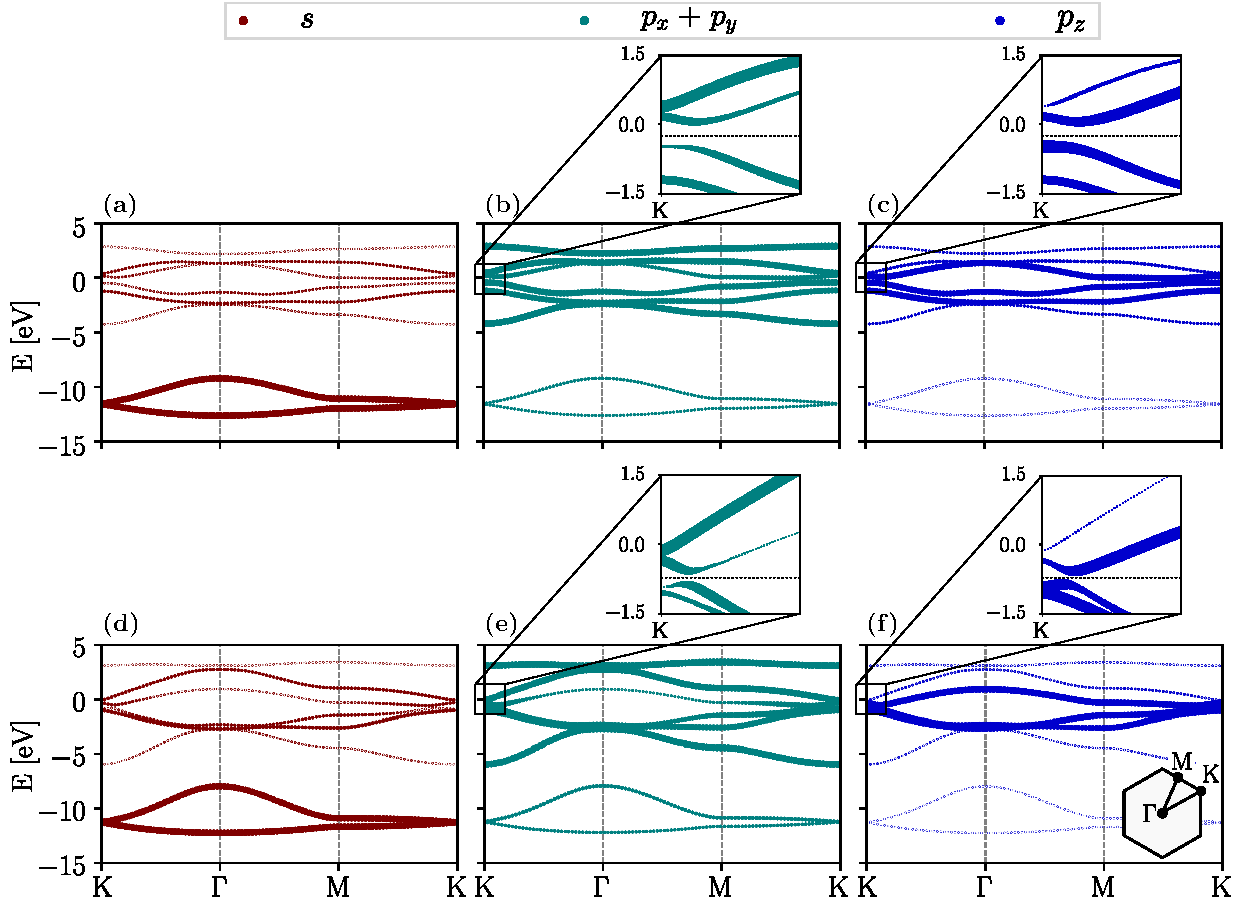
\includegraphics[width=\textwidth]{tci_bs_flat.pdf}
\caption[Orbital-projected band structures of free-standing bismuthene and antimonene]{Orbital-projected band structures of \textbf{(a, b, c)} bismuthene and \textbf{(d, e, f)} antimonene. Valence bands maxima (composed mostly of $p_z$ orbitals) and conduction bands minima (with contributions from all $p$ orbitals) are located close to the $K$ point.}
\label{fig:bs-anti-bism}
\end{figure}

\section{Coupling to SiC substrate}
\label{sec:sic}
A substrate provides mechanical support to deposited layers. However, it may also interact with the layers and greatly influence their properties. Here, we investigate the effect of SiC substrate on bismuth and antimony layers, which is effectively described by shifting the energy of out-of-plane $p_z$ orbitals away from the low-energy sector~\cite{Reis287}. We calculate the energy gap while changing the value of energy of $E_{p_z}$ orbitals (but keeping $E_{p_x}$ and $E_{p_y}$ energies fixed) as illustrated in Fig.~\ref{fig:egap-substrate}. We note that within this TB model, it is not possible to define the Fermi level at intermediate values of $E_{p_z}$ when the bands are continuously shifting in energy with respect to $E_{p_z}$. Therefore, we exclude the parameter region around $E_{p_z} \sim - 2$ eV (denoted by a yellow color) from the phase diagrams. The determined band gaps for bismuthene and antimonene are, respectively, $E_{gap} \sim 0.9$ eV and $E_{gap} \sim 0.34$ eV, comparable with DFT results from Ref.~\cite{Hsu_2015} with structures on the top of SiC under different tensile strains. The energy gap in bismuthene is almost three times larger than the gap in antimonene as well the gap of a bismuth monolayer, $E_{gap} = 0.25$ eV, which was noticed in Ref.~\cite{Reis287}. In addition, we show that a weak coupling to the substrate is sufficient to observe a transition from the TCI to a TI phase, which occurs around $E_{p_z} \sim - 2.5$ eV in both structures. After a topological phase transition, the energy gap is stable and only slightly affected by the coupling strength with the substrate.

\begin{figure}[H]
\centering
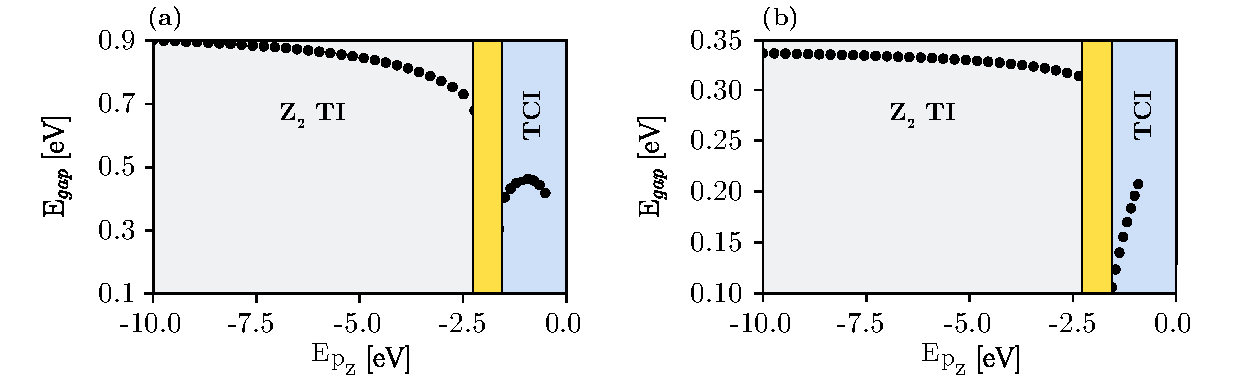
\includegraphics[width=\textwidth]{tci_egap-substrate.pdf}
\caption[Energy gap $E_{gap}$ as function of interaction with a substrate]{Energy gap $E_{gap}$ as function of interaction with a substrate modelled by changing of energy $E_{p_z}$ of $p_z$-orbitals for \textbf{(a)} bismuthene and \textbf{(b)} antimonene. Free-standing monolayer of bismuthene (antimonene) has $E_{p_z}= - 0.486$ eV ($ E_{p_z} = - 0.926$ eV), see Table~\ref{tab:TB}. $E_{p_z} = - 10$ eV corresponds to the structures deposited on the SiC substrate. The yellow areas refer to $E_{p_z}$ values with a not-well defined Fermi energy coinciding with transition regions from TCI to TI phases.}
\label{fig:egap-substrate}
\end{figure}

We consider also a transition between a buckled bismuth (antimony) monolayer and bismuthene (antimonene) by applying additional strain for structures deposited on the substrate. The coupling to the SiC substrate of buckled structure is modeled by shifting the energy $E_{p_z}$ of $p_z$ orbitals for an upper atom from a unit cell, while a lower atom has the energy of $p_z$ orbital $E_{p_z} = - 10$ eV as it is fully coupled to the substrate for all strain values. In Fig.~\ref{fig:free-substrate-bisb}, we show that layers deposited on a substrate are topologically trivial. It is observed that a small strain (around $1 \%$ for Bi and $4\%$ for Sb) induces a transition to a TI phase. With a larger strain, the band gap monotonically increases up to the largest value at $20\%$ strain corresponding to flat structures.

\begin{figure}[H]
\centering
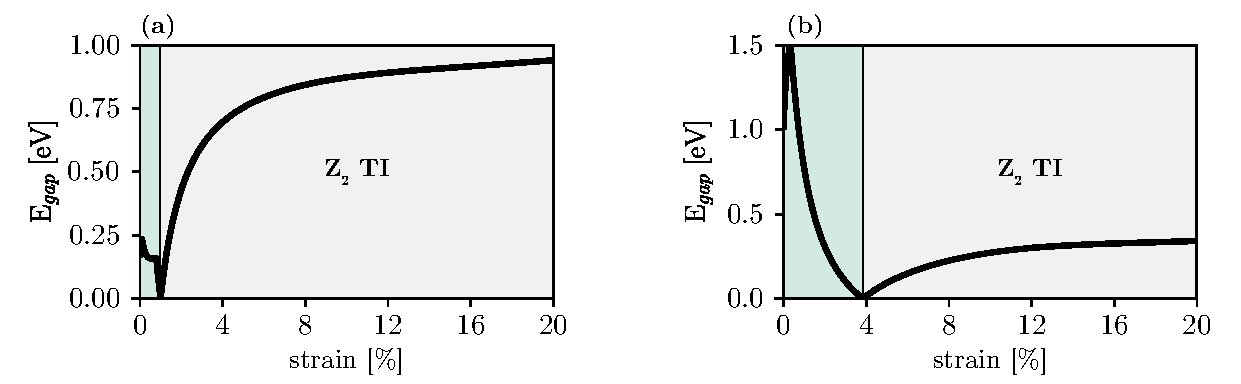
\includegraphics[width=\textwidth]{tci_gap-sub-strain.pdf}
\caption[Energy gap $E_{gap}$ as a function of strain for bismuth and antimony monolayers deposited on the SiC substrate]{Energy gap $E_{gap}$ as a function of strain for \textbf{(a)} bismuth and \textbf{(b)} antimony monolayers deposited on the SiC substrate. Unstrained structures are within topologically trivial phase, however a small strain ($ \sim 1 \%$ for Bi and $\sim 4\%$ for Sb) leads to a transition to TI phase regime (denoted by a gray background) which is observed over all investigated strain range. At $20\%$ strain, the systems are completely flat.}
\label{fig:egap-substrate-strain}
\end{figure}

Finally, in Fig.~\ref{fig:free-substrate-bisb} we compare the entanglement spectra for the systems in distinct topological phases.

\begin{figure}[H]
\centering
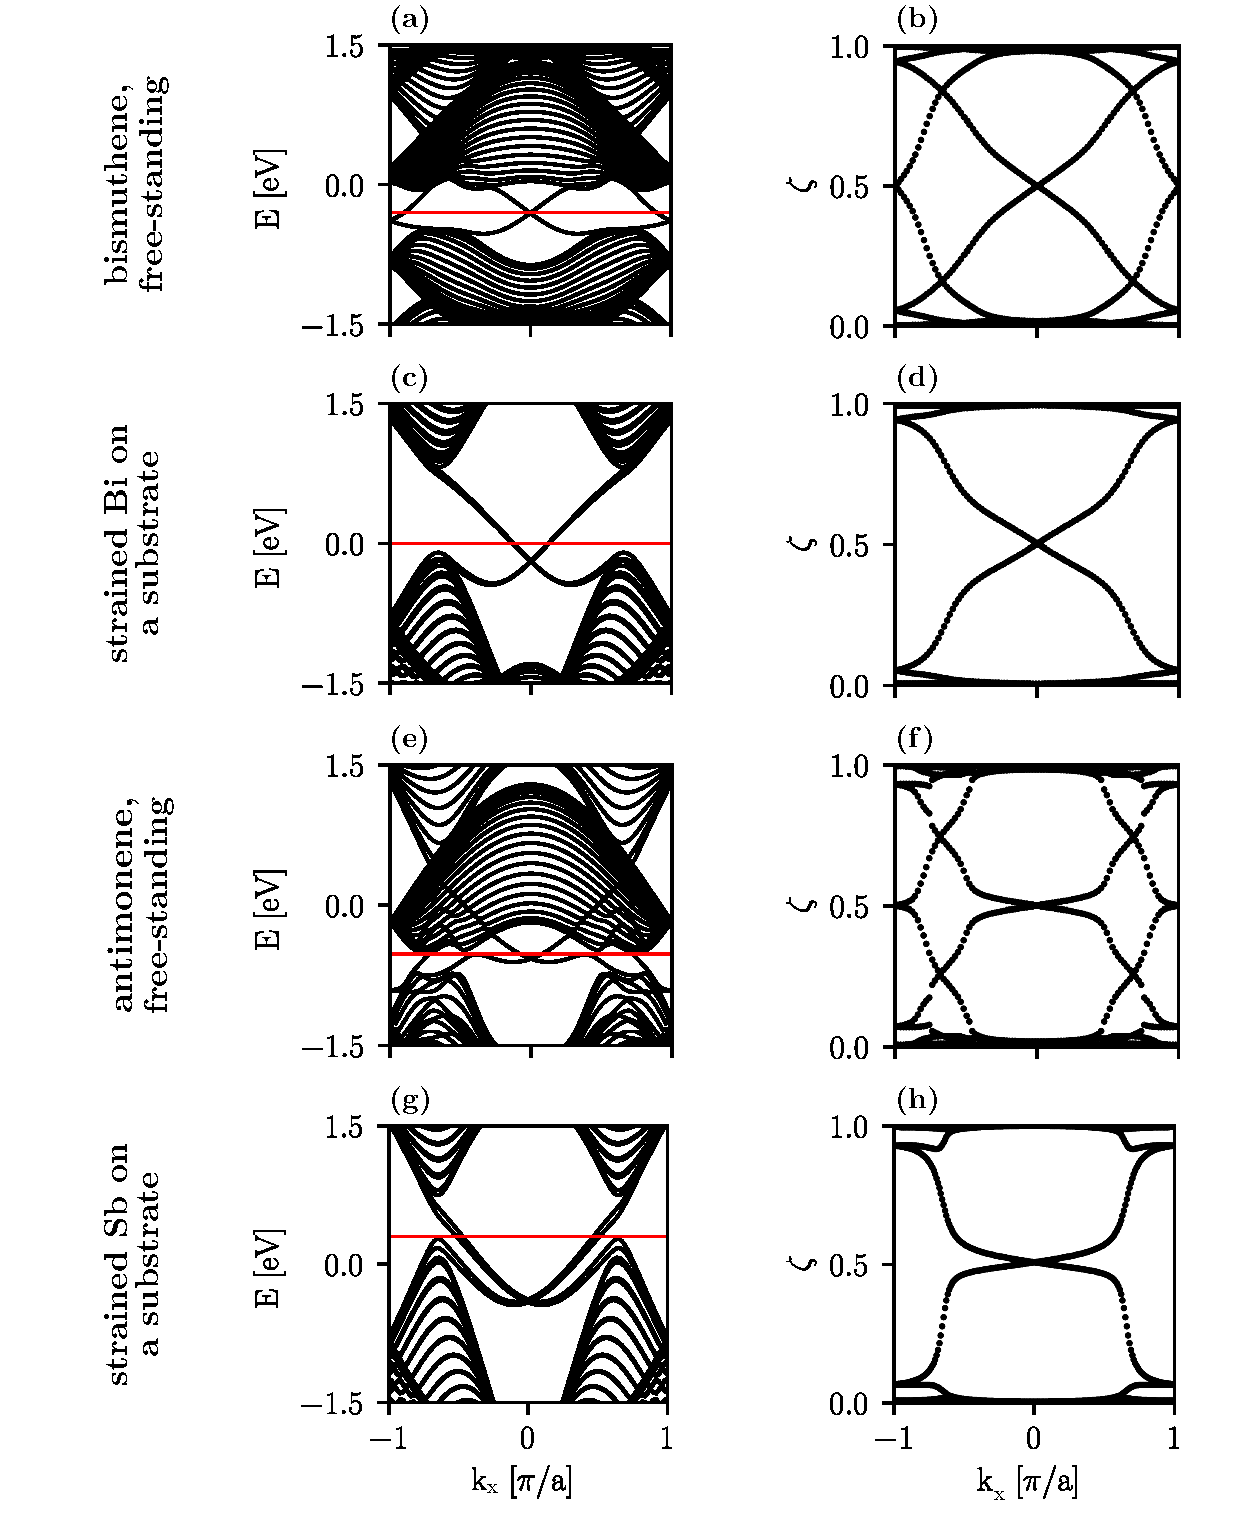
\includegraphics[width=0.85\textwidth]{tci_bands_flat.pdf}
\caption[Comparison of energy and entanglement spectra of the systems in TI and TCI insulating phases]{Energy spectra around the Fermi level (denoted by a red line) and corresponding entanglement spectra of free-standing \textbf{(a, b)} bismuthene  and  \textbf{(e, f)} antimonene, together with monolayers of \textbf{(c, d)} bismuth and \textbf{(g, h)} antimony within a TI phase at $12.5 \%$ strain on the SiC substrate in a ribbon geometry. The interaction with the substrate splits the double degeneracy of each branch of edge states. The degeneracy of these edge states is removed due to inversion-symmetry breaking as two atoms from a unit cell couple differently to the substrate. Distinct topological phases can be distinguished by the number of branches spectrally connecting 0’s and 1’s eigenvalues in the entanglement spectrum: there are two pairs of modes in the TCI phase with crossings at $k_x = 0, \, \pi$ (see \textbf{(b)} and \textbf{(f)}) and one pair of modes in the TI phase, which crosses at $k_x = 0$ (in \textbf{(d)} and \textbf{(h)}).}
\label{fig:free-substrate-bisb}
\end{figure}

For free-standing bismuthene and antimonene, the ES has two pairs of modes exhibiting spectral flow, which is in an agreement with computed mirror Chern number. In contrast, a single crossing of two modes in the ES is a feature of strained monolayers of Bi and Sb on the substrate exhibiting the TI phase.